\input{../header}
\usepackage{pgfplots}
\usetikzlibrary{positioning,matrix,arrows}

\begin{document}
%


%\onehalfspacing
\allowdisplaybreaks
%##################################################################
\section{The bottle problem}

The water level in a bottle is related to the amount of water that's in the bottle.

\begin{enumerate}[leftmargin=*]

\item First, let's think about the \textbf{quantities} in this problem. A quantity is a thing that you can measure, with numbers and units. Quantities that \textit{change} are called \textbf{variables}:

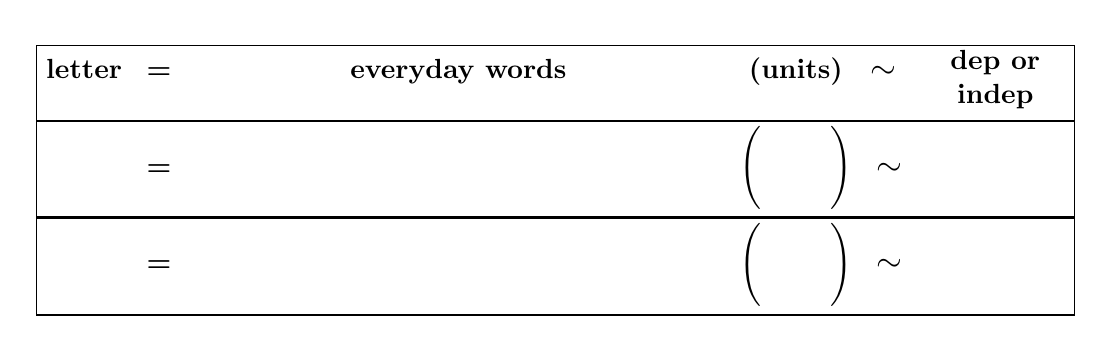
\begin{tikzpicture}
    \matrix (v) 
        [matrix of nodes,
        nodes={
            align=center,
            font=\bfseries
        },
        minimum height=3.5em,
        minimum width=2em,
        text depth=1ex,
        text height=2ex,
        nodes in empty cells,
        row 1/.style={minimum height=1.5em},
        column 3/.style={text width=0.55\linewidth},
        column 6/.style={text width=5em}
        ]
    {
        letter& =& everyday words& (units)& {\large$\sim$} & 
        |[text depth = 1.5em, anchor=center]| dep or indep\\
        \phantom{letter}&=&&\Bigg(\phantom{units}\Bigg)&{\large$\sim$}&\\
        \phantom{letter}&=&&\Bigg(\phantom{units}\Bigg)&{\large$\sim$}&\\
    };
    \draw[black] (v-1-1.north west) rectangle (v-1-6.south east);
    \draw[black] (v-2-1.north west) rectangle (v-2-6.south east);
    \draw[black] (v-3-1.north west) rectangle (v-3-6.south east);
\end{tikzpicture}
\item Now let's think about \textbf{function notation}. If volume is measured in cups and height is measured in inches, what does the equation \( h(3) = 5\) mean?

\vspace{0.5in}

\item Explore the following claim: Steepness of the graph of the function $h(V)$ has something to do with the cross-sectional area of the bottle.

\vfill
\vfill

\item What bottle shapes could correspond to a straight-line graph? Do the sides have to be straight?
\vfill

\item Draw the graph for a pint glass that gets \textbf{wider} as you go up, and draw the graph for a volcano vase that gets \textbf{narrower} as you go up.

\vfill

\item What's the deal with a bottle that changes from getting narrower to getting wider? Or one that changes from getting wider to getting narrower?

\vfill

\end{enumerate}
\end{document}